\documentclass[a4,center,fleqn]{NAR}
\usepackage{hyperref}
\usepackage{graphicx}
\usepackage{csquotes}
\usepackage{amsmath}
\usepackage{setspace}
\usepackage{float}
\usepackage{caption}
\usepackage{subcaption}
\usepackage[super]{nth}
\usepackage{multirow}
% Enter dates of publication
\copyrightyear{2017}
\pubdate{18 March 2017}
\pubyear{2017}
\jvolume{37}
\jissue{12}

\usepackage{tikz}
\usetikzlibrary{shapes}
\usetikzlibrary{positioning}
\usetikzlibrary{arrows}
\usetikzlibrary{fit}
\usetikzlibrary{decorations.pathreplacing}
\usetikzlibrary{shadows.blur}
\usetikzlibrary{shapes.symbols}

%\articlesubtype{This is the article type (optional)}

\begin{document}
\title{HiC Contact Map Comaprison Using Graphlet Approach}

\author{%
    Behnam Rasoolian\,$^{1,*}$,
    Debswapna Bhattacharya\,$^{1}$
    \footnote{
    Tel: +1 334 5212814; Email: bzr0014@auburn.edu}}

    \address{%
        $^{1}$ Auburn University
        }
        % Affiliation must include:
        % Department name, institution name, full road and district address,
        % state, Zip or postal code, country

%        \history{%
%            Received January 1, 2009;
%            Revised February 1, 2009;
%            Accepted March 1, 2009}

            \maketitle

\begin{abstract}

In this study, we investigated
dissimilarities between normal cells and cancerous cells,
through analyzing HiC contact maps. 
Our results show that certain orbit distributions
have significanly higher correlation 
between Leukemic cells.

\end{abstract}

\section{Introduction}

Ideally, it is desirable to compare 3D structures of 
cell in order to make such comparisons.
However, the main challenge is that 
3D structure of a cell is not readily available. Based on
\cite{adhikari2016chromosome3d}, fluorescence in situ hybridizaiton
(FISH) is used for investigating 3D configuration of chromosomes.
However, this method can only be used locally and cannot map
the whole structure of the chromosomes.
In orther to find dissimilarities in the 3D structure of 
chromosomes, we used HiC dataset.
The HiC method, which was developed by 
\cite{lieberman2009comprehensive}, captures interactions between 
chromosomal fragments in kilobase resolution. Based on HiC data, an
\textit{interaction frequency (IF) } matrix can be developed 
between \textit{loci} at a desired resolution.
A cell $IF_{ij}$ in an interaction frequency matrix captures 
the number of interaction detected
in HiC dataset between locus $i$ and locus $j$ in the genome.
An interaction matrix can be used to develop both 
inter- and intra-chromosomal interaction matrices.
We believe differences in interaction matrices can 
be found between normal cells and cancerous ones.

Graphlet comparison is a novel method used to compare 
large networks in order to
find local similarities in them.
Authors of \cite{prvzulj2007biological} 
provide a new measure of PPI
network comparison
based on 73 constraints. This is used in order to compare two large
networks in order to detect similarities.

In \cite{milenkoviae2008uncovering} the authors
 provide heuristics to compare two nodes in a graph
based on signature vectors, which are 73-dimensional vectors
$\mathbf{s}^T
= [s_0, s_2, ..., s_{72}]$ where $s_i$ denotes the number of nodes in
the network that are part of an orbit $i$. \\
They concluded that proteins with similar surroundings perform
similar functions.

In \cite{milenkovic2010cancer}, the same author investigates 
cancer-causing genes to find similarities in their signatures. After
clustering the genes based on \textit{signature similarity} criteria,
some clusters contain a lot of cancerous genes.
They use 4 different clustering methods with varying parameters to cluster
the proteins. They then predict the cancer-relatedness of a protein 
$i$ using
an enrichment criteria $\frac{k}{|C_i|}$ where $C_i$ is the cluster
where protein $i$ belongs and $k$ is the number of cancer-causing
proteins in $C_i$ and $|C_i|$ is the size of $C_i$.


The authors of \cite{di2010fast} generalized the idea of graphlets to 
ordered graphs were the nodes are labeled in ascending order.
As can be viewed, there are a total of 14 orbits for graphlets of size
2 and 3 since the label of graphlets is also included in toplogy.
In the new definition, $d_v^i$ denotes the number of orbit $i$ touches 
node $v$. Each node, is then assigned a vector of length 14 
\footnote{number of orbits in graphlets of size 2 and 3}
$(d_v^1, d_v^2, ..., d_v^{14})$ 
and similarity of two nodes in two contact maps can be compared by
how geometrically close their corresponding vectors are.

\subsubsection{Notations}
In this paper, matrices and vectors are represented with bold
capital and bold small letters respectively.
matrix rows and columns are represented by a \textit{dot}
notation. For example, the $i$th row of matrix $M$ is
denoted by $M_{i.}$ and its $j$th column is represented
by $M_{.j}$.

We denote the set of all contact maps in cell line $T$ with 
$\mathbb{C}^T$. If no particular cell line is addressed, the
subscripts are dropped.
Any arbitrary member of $\mathbb{C}$ is denoted by 
$C_{ij}$, where $i$ and $j$ ($j \ge i$) represent the two chromosomes involved. 
In human cells this set contains a total of 276 contact maps,
23 of which are intra-chromosomal and the rest are inter-chromosomal.
For ease of representations, intra-chromosomal contact maps are
distinguished by a single superscript, so we have $C_{i,i} =
C_i$.

We denote the number of loci in a chromosome $i$ by $N_i$.
The set of all loci involved in contact map $C_{ij}$ is denoted 
by $\mathbb{V}_{ij}$.
In intra-chromosomal contact maps, $\mathbb{V}_{i,i}$ containts only the 
loci of that particular chromosome ($|\mathbb{V}_i| = N_i$), while in 
inter-chromosomal contact maps $\mathbb{V}_{ij}$ contains the loci in
the both of chromosomes involved ($|\mathbb{V}_{ij}| = N_i + N_j$).

% **************************************************************
% Keep this command to avoid text of first page running into the
% first page footnotes
\enlargethispage{-65.1pt}
% **************************************************************

\section{Materials and Methods}
We re-used Leukemic Hi-C libraries 
created in \cite{wang2013properties}
These libraries we sequenced 
for cases of primary human B-acute
lymphoblastic leukemia (B-ALL or ALL), 
the MHH-CALL-4 B-ALL cell
line (CALL4), 
and the follicular lymphoma cell-line (RL).
Just as \cite{wang2013properties}, 
we used normal B-cell line (GM068990)
from \cite{lieberman2009comprehensive} 
for our comparisons.
We created contact maps of resolution
500kb and normalized it using 
the \texttt{iced} package in python
developed by \cite{servant2015hic}.



\subsection{Thresholding contact maps}
In order to be able to extract graphlets, HiC contact maps should be modeled as
unweighted graphs where the nodes represent the loci and an edge between two 
nodes represent a \textit{significant} interaction between the loci.
This can be achieved by thresholding the contact maps. The result
of the thresholding procedure is a binary matrix which also can serve as
an adjacency matrix for an unweighted, undirected graph. The graph can then be
used for orbit extraction.

When thresholding contact maps, it is necessary to make sure
that both global and local features are maintained. We could consider 
thresholding the contact maps by simply setting values above a fixed value to
one and the rest to zero; However, in practice, this method resulted in graphs
that capture the local structure of the contact maps poorly. This is because
intensities follow an exponential distribution with a mean close to zero
with a few very larges values that correspond to interactions along 
or close to the main diagonal of the contact maps.
Thus, picking relatively large numbers would result in ignoring interactions
that are far from the main diagonal while picking small values will lead to
capturing too many (insignificant) interactions.

To the best of our knowledge, little work has dealt with the task of
thresholding HiC contact maps. There has been some statistical approaches
developed on similar data in other fields. 
For example, authors of \cite{ginestet2011statistical} developed 
Statistical Network (SPN) analysis
where the choice of thresholding value is made by statistical inference.
This method, although very robust, works within the framework of 
design of experiments where the same
network can be extracted for different 
individuals under different treatments. Thus a relatively large
set of different contact maps need to be available in order for
this method to be applicable towards our end.

Instead, in order to threshold the matrix so that both global and local patterns are
captured, we borrowed the concept of \textit{adaptive thresholding} from image 
processing context. In this method, in order to be set, a pixel should have
an intensity larger than the average of non-zero intensities in its
\textit{neighborhood}. The neighborhood is defined by a sliding kernel 
that passes through the contact map with the pixel at its middle at 
each step. Figure \ref{local_thresholded_chr1_chr1} demonstrates result of 
this thresholding approach for intra-chromosomal contact maps of chromosome 1.
Refer to supplementary material for all 23 interchromosomal thresholding
results.
\begin{figure}[t]
    \centering
    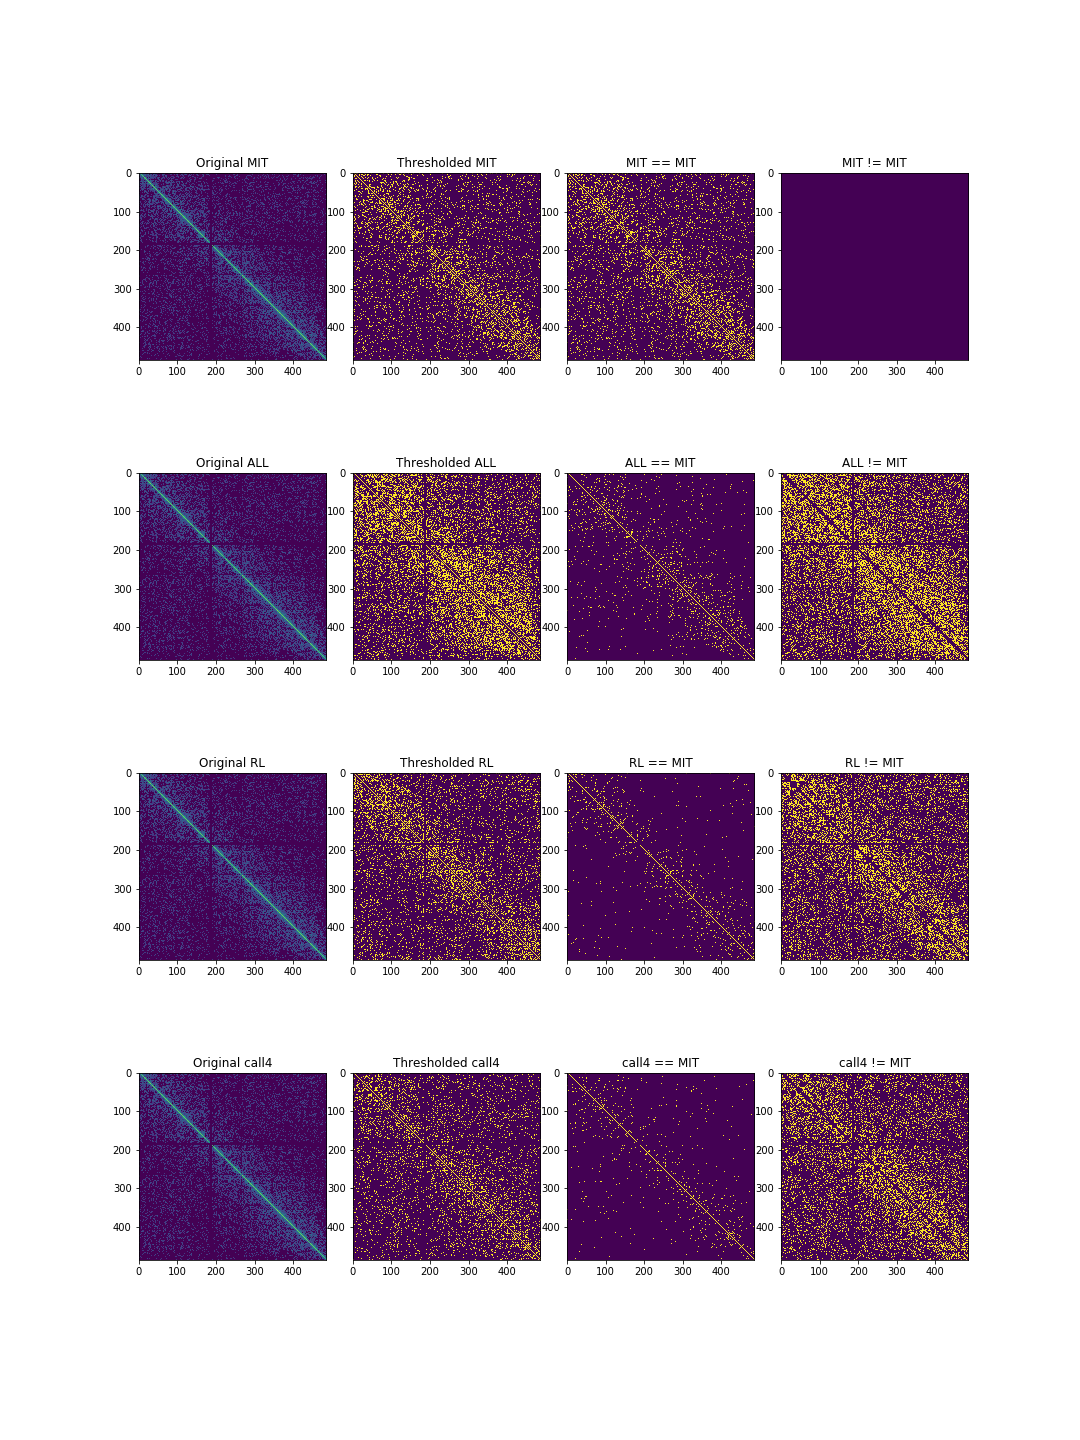
\includegraphics[width=.5\textwidth]{figures/local_thresholded_chr1_chr1.png}
    \caption{Result of thresholding interchromosomal contact map of chromosome 1
    using a kernels of size $5 \times 5$ for all cell lines. 
    The first row shows the thresholded
    maps. Second and third rows demonstrate pair-wise similarities and 
    differences between contact maps respectively.}
    \label{local_thresholded_chr1_chr1}
\end{figure}

\subsection{Orbit Extraction}
Once the thresholded contact maps are obtained, graphlets and orbits can be 
extracted. We used the \texttt{orca} package in \texttt{R} programming 
language to extract the graphlets. As a result of graphlet extraction, 
For each loci in each contact map, a \textit{signature vector} of size
73 is created. Thus for each cell line, we would have 276 
\textit{signature matrices} of
size $|V^{ij}|\times 73$, where $V^{ij}$ is the number of loci
involved in contact map between chromosomes $i$ and $j$. Figure
\ref{fig:graphlet_extraction} illustrates the process and results
of signature matrix extraction schematically.
\begin{figure}
    \centering
    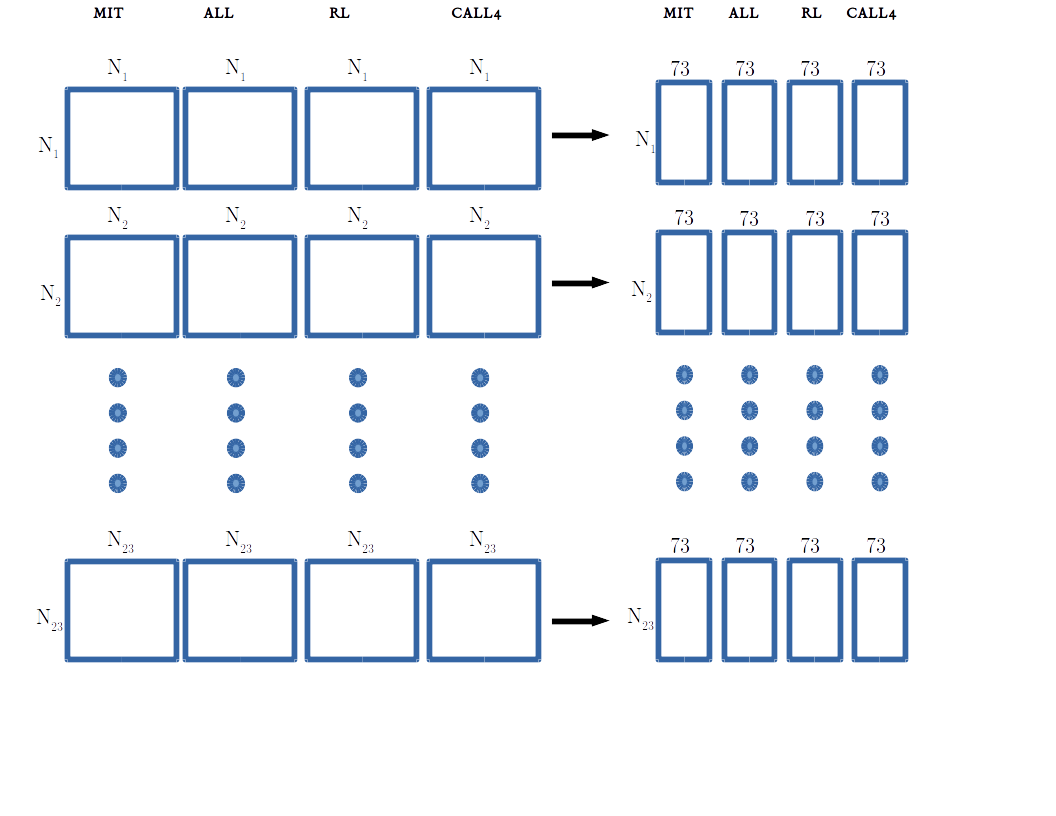
\includegraphics[width=.5\textwidth]{figures/graphlet_extraction.png}
    \caption{Graphlet extraction for the four cell lines. For each
    loci in each contact map between chromosomes $i$ and $j$, 
    the signature vectors of length 73 are extracted, resulting 
    in a \textit{signature matrix} of size $|V^{ij}| \times 73$,
    where $V^{ij}$ 
    is the number of loci involved.}
    \label{fig:graphlet_extraction}
\end{figure}

For a particular
$\mathbf{C}_{ij}$, we denote $\mathbf{S}_{ij}$ as its \textit{signature 
matrix}. Each cell $S_{ijlo}$ in $\mathbf{S}_{ij}$ captures how many
times loci $l$ in $\mathbf{C}_{ij}$ occured as part of orbit $o$.


\begin{figure}
    \centering
    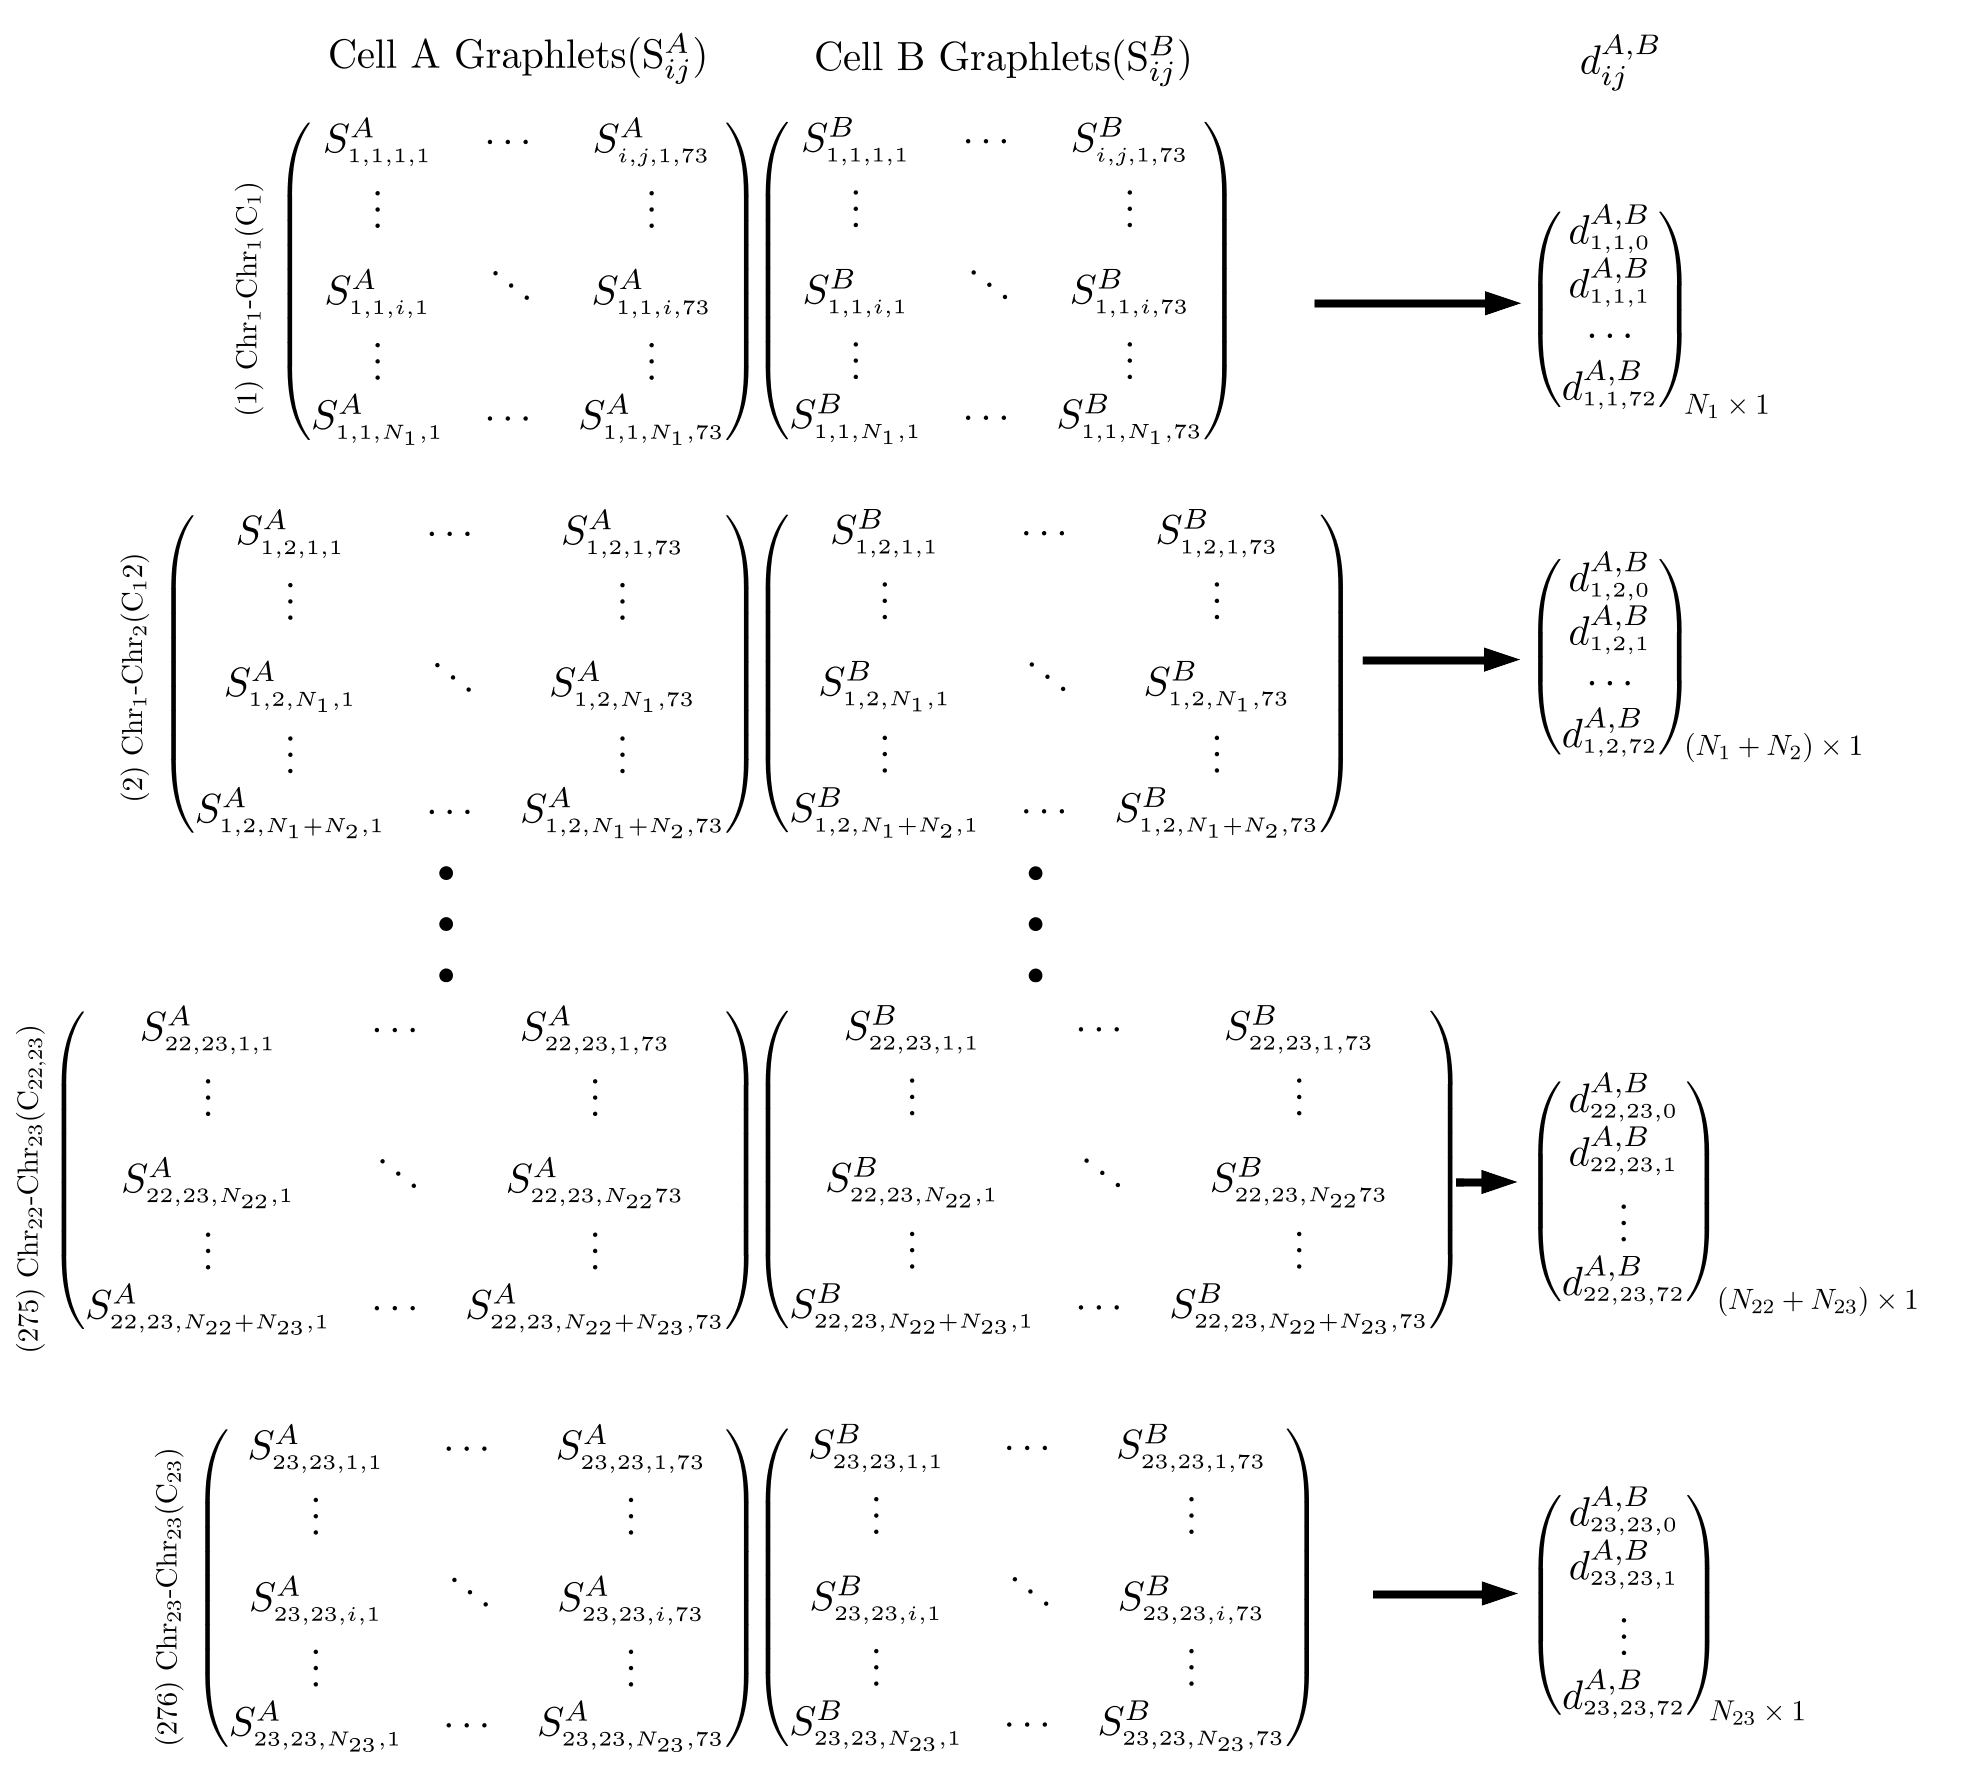
\includegraphics[width=.5\textwidth]{figures/graphlet_distance_schema.png}
    \caption{Calculating pair-wise loci distances. For each loci (row) 
    in each
    contact map in MIT cell line, its distance is calculated based on
    equation \ref{eq:distance_total} with the corresponding loci in
    leukemic cells. The result of this process is a 
    \textit{signature distance vector} of size
    $|V^{ij}| = N_i+N_j$ for each contact map.
    }
    \label{graphlet_distance_schema}
\end{figure}
\begin{figure}
    \centering
    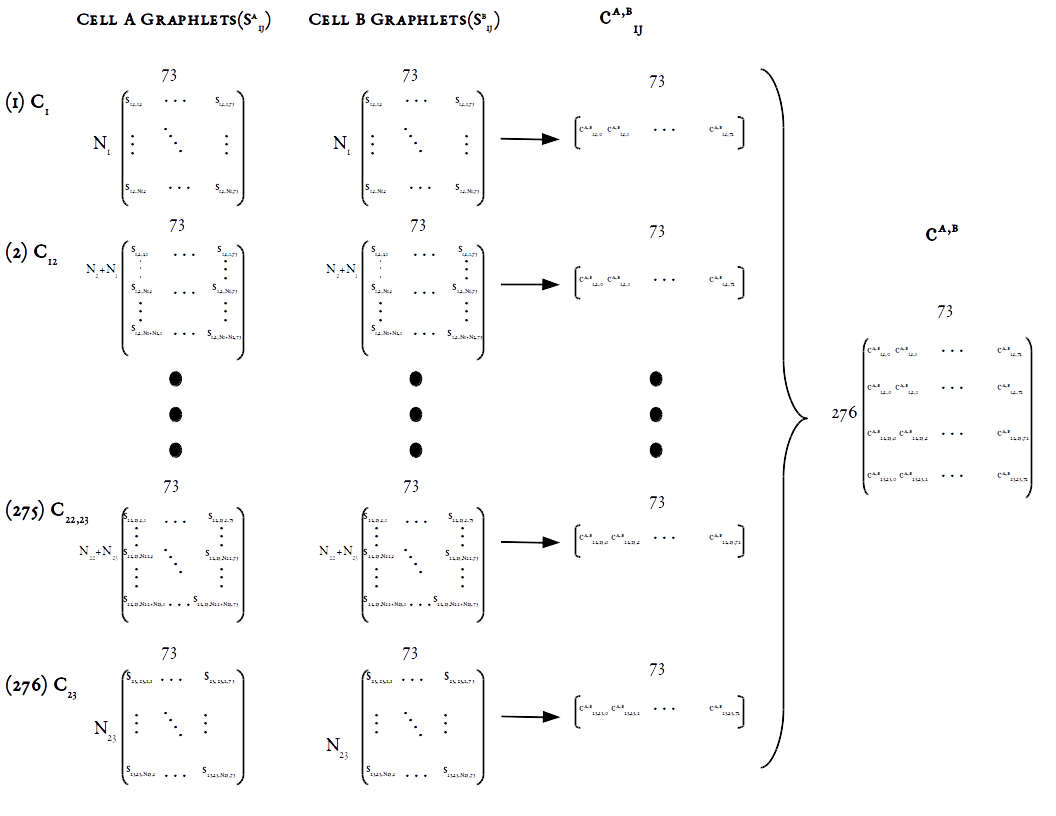
\includegraphics[width=.5\textwidth]{figures/graphlet_correlation_schema.png}
    \caption{Calulating pair-wise orbit correlations. For each orbit (column)
    in each contact map in MIT cell line, its correlation with the
    same orbit in the same contact map 
    in leukemic cells is calculated. The result of
    this process is a \textit{signature correlation} vector of size
    73 which captures how similar frequencies of two orbits are.
    In order to test our second hypothesis, we calculated averages
    across contact maps (along the vertical red arrow) to test 
    hypothesis \ref{eq:h2a}
    and across orbits
    (along the horizontal red arrows) to test hypothesis \ref{eq:h2b}.}
    \label{graphlet_correlation_schema}
\end{figure}
%$
%\begin{pmatrix}
%    {S}^A_{\scriptscriptstyle i,j,1,1}         &
%    \cdots                                     &    
%    {S}^A_{\scriptscriptstyle i,j,1,72}        \\
%%%%%%%%%%%%%%%%%%%%%%%%%%%%%%%%%%%%%%%%%%%%%%%%%%%%%
%    \vdots                                     &                
%                                               &      
%    \vdots                                     \\
%%%%%%%%%%%%%%%%%%%%%%%%%%%%%%%%%%%%%%%%%%%%%%%%%%%%%
%   {S}^A_{\scriptscriptstyle i,j,N_1,1}    &
%   \ddots                                            &    
%   {S}^A_{\scriptscriptstyle i,j,N_1, 72} \\
%%%%%%%%%%%%%%%%%%%%%%%%%%%%%%%%%%%%%%%%%%%%%%%%%%%%%
%    \vdots                                     &                
%                                               &      
%    \vdots                                     \\
%%%%%%%%%%%%%%%%%%%%%%%%%%%%%%%%%%%%%%%%%%%%%%%%%%%%%
%   {S}^A_{\scriptscriptstyle i,j,N_1+N_2,1}   &
%    \cdots                                &
%   {S}^A_{\scriptscriptstyle i,j,N_1+N_2, 72}
%\end{pmatrix}
%$
%
%$
%\begin{pmatrix}
%    {C}^A_{\scriptscriptstyle i,j,1,1}     &
%    \cdots    &
%    {C}^A_{\scriptscriptstyle i,j,1,N_1} \\
%%%%%%%%%%%%%%%%%%%%%%%%%%%%%%%%%%%%%%%%%%%%%%%%%%%%%
%    \vdots                             &
%    \ddots&
%    \vdots                             \\
%%%%%%%%%%%%%%%%%%%%%%%%%%%%%%%%%%%%%%%%%%%%%%%%%%%%%
%    {C}^A_{\scriptscriptstyle i,j,N_1,1}   &
%    \cdots&                  
%    S^A_{\scriptscriptstyle i,j,N_1, N_1}
%%%%%%%%%%%%%%%%%%%%%%%%%%%%%%%%%%%%%%%%%%%%%%%%%%%%%
%\end{pmatrix}
%$

%We divided the task of graphlet comparison into two parts: first we compare
%graphlets from each contact map in normal cell lines (MIT) with the 
%same contact maps in the other three Leukemic cells. Second we compare 
%contact maps in a similar way but this time only between leukemic cells.
%In the former case, the null hypothesis is that there is no difference
%between contact maps of normal cells and leukemic cells and in the latter
%case, the null hypotheis is that there is no difference between 
%different leukemic cells.

We consider two measures of \textit{difference} when comparing contact
map graphlets across cell lines. 
The first measure is \textit{signature distance vectors} between
each contact map of two cell lines. 
For a pair of cells A and B, let 
$\mathbf{S}^A_{ij}$  and $\mathbf{S}^B_{ij}$ be their
signature matrices. The \textit{signature distance} of
contact map $\mathbf{C}_{i,j}$ between A and B is denoted
by $\mathbf{d}^{\scriptscriptstyle A,B}_{ij}$. $\mathbf{d}^{\scriptscriptstyle A,B}_{ij}$ 
is a vector of size $|V_{i,j}|$
and its elements $d^{\scriptscriptstyle A,B}_{i,j,l}$ are
calculated using the following formula from \cite{prvzulj2007biological}:

\begin{equation}
    d^{\scriptscriptstyle A,B}_{i,j,l} = 
    \frac{1}{73}\sqrt{\sum_{o=0}^{72}{t_{lo}^2}}
    \label{eq:distance_total}
\end{equation}

where elements of $t_{i,j,l,o}$ is the
distance between each
loci (row) $l$ in $\mathbf{S}^A$ and the the same loci in 
$\mathbf{S}^B$ for
orbit $o$ as is calculated as below:

\begin{equation}
    t_{lo} = w_o \times 
    \frac{log(S_{ijlo}^A+1) - log(S_{ijlo}^B+1)}
    {log(max(S_{ijlo}^A, S_{ijlo}^B) + 2)}
    \label{eq:distance_single}
\end{equation}


This process is illustrated in Figure \ref{graphlet_distance_schema}.
Using this distance measure, we can quantify how two loci are close to
each other in terms of local neighborhood between the two contact maps.

The second measure of comparison that we use captures how 
similar two orbits are in terms of their count 
frequencies across loci between two contact maps. 
Each column in $S_{ij}$ can provide information
regarding the \textit{frequency distribution} of orbits throughout
the contact map $C_{ij}$. 
We can find how similar these distributions are to each other using
correlation measures.
These correlations are denoted by $\mathbf{m}^{\scriptscriptstyle A,B}_{i,j}$ and
can be calculate using
any plausible correlation measure. 
In this study, for each contact map,  we calculated
similarity between orbit distributions using Pearson's r 
correlation, which is computationally efficient.
However, pearson's r might not be able to capture
non-functional relationships between distributions. As a result, we
also used Maximal Information Coefficient (MIC) 
\cite{reshef2011detecting} in order to compare
correlations. MIC calculates mutual information (MI) between two
distributions, but utilizes dynamic programming in order adjust
bin sizes and numbers in order to achieve highest MI.
MIC values between two variables fall between 0 and 1,
with 0 meaning the two variables are completely independent
and 1 meaning one is dependant on the other.
We used both Pearson's r and MIC in order to compare orbit
frequencies. Although results from both approaches were more
or less consistent, MIC showed higher robustness than Pearson's 
r method.

If MIC is used as correlation measure, each element of 
 $\mathbf{c}$ is calculated as below:
\begin{equation}
    m^{\scriptscriptstyle A,B}_{ijo} = MIC(\mathbf{S}^A_{ij.o}, \mathbf{S}^B_{ij.o})
    \label{eq:mic}
\end{equation}
Alternatively, if we use Pearson criterion we would have:
\begin{equation}
    m^{\scriptscriptstyle A,B}_{ijo} = Pearson(\mathbf{S}^A_{ij.o}, \mathbf{S}^B_{ij.o})
    \label{eq:pearson}
\end{equation}

\section{results and discussions}

\begin{figure*}
    \centering
    \begin{subfigure}[b]{\textwidth}
        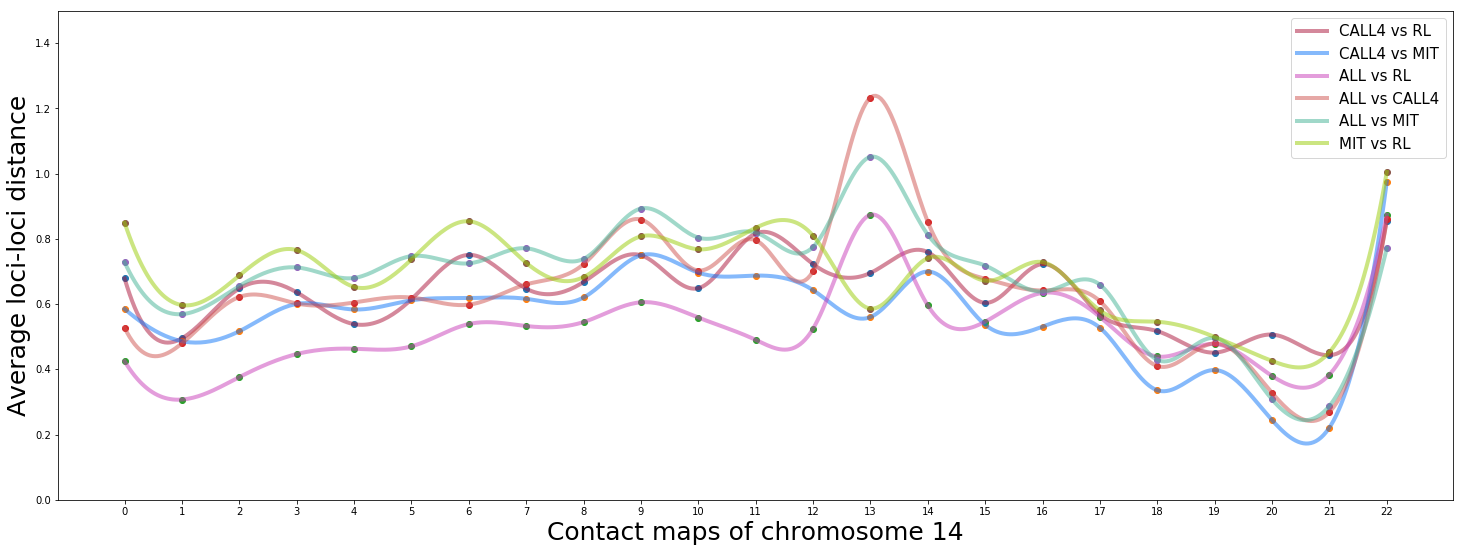
\includegraphics[width=\textwidth]{figures/orbit-distances_chr14.png}
        \caption{}
        \label{fig:orbit-distances_chr14}
    \end{subfigure}
    \begin{subfigure}[b]{\textwidth}
        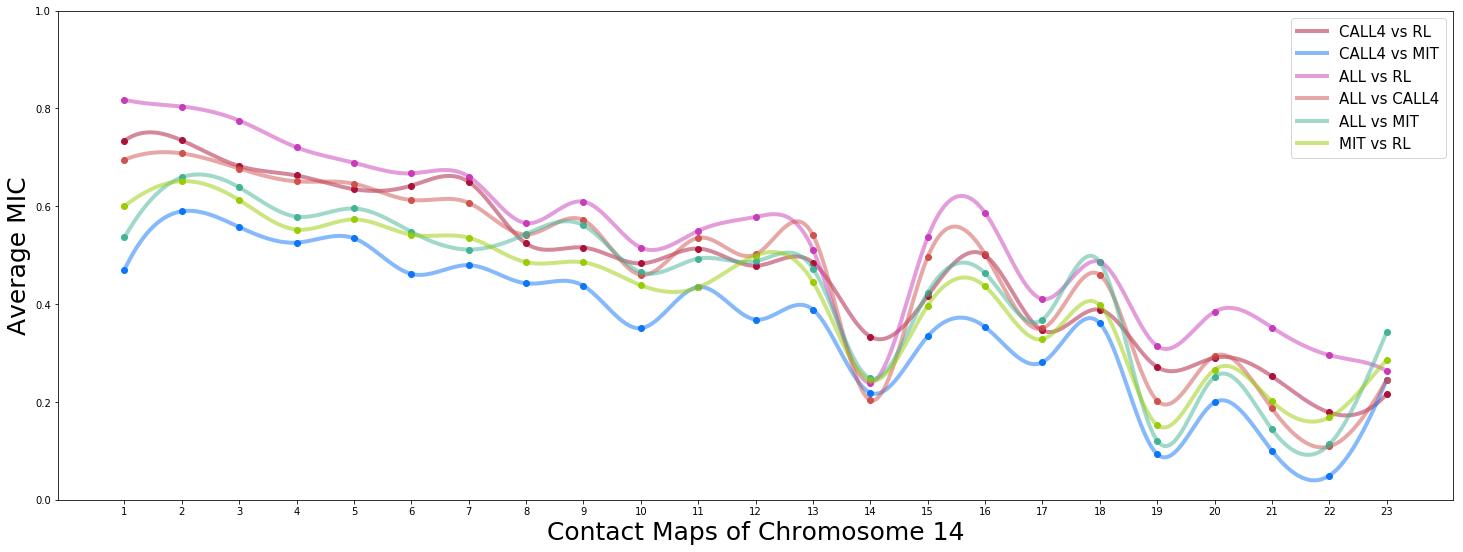
\includegraphics[width=\textwidth]{figures/contact_maps_correlations_chr14.png}
        \caption{}
        \label{fig:contact_maps_correlations_chr14}
    \end{subfigure}
    \caption{   
        \textbf{(a) Pair-wise graphlet signature difference for
        all 276 contact maps:}
        Each point on a graph is the result of averaging all
        the distances across all loci of that contact map.
        ($\bar{\mathbf{d}}^{\scriptscriptstyle A,B}_{i,j} \quad
        \forall i,j \in \{1 ... 23\} \quad \& \quad j \ge i$).  
        \vspace{.1cm} \\
        \textbf{(b) pair-wise average contact map orbit correlations
         for all contact maps:}
        ($\bar{\mathbf{m}}^{\scriptscriptstyle \scriptscriptstyle A,B}_{i,j} 
        \quad \forall i,j \in \{1 ... 23\} \quad \& \quad j \ge i$:
        average along the red \textit{vertical} arrow in figure 
        \ref{graphlet_correlation_schema}).
        These values are calculated by averaging over 
        pairwise correlations of orbits of
        $\mathbb{Q}$ in a contact map.
     }
    \label{fig:results_all}
\end{figure*}

Result of pair-wise contact map graphlet distances is
illustrated in supplementary materials. 
As an example, we plotted average
distances only for chromosome 
14 in Figure \ref{fig:orbit-distances_chr14}.
Each point on the graph is the
average of the graphlet distance vector 
of the two cell lines specified in the legend
($\bar{\mathbf{d}}^{\scriptscriptstyle A,B}_{i,j}$).

By comparing signature distance vectors, one can find
how contact maps
differ from each other in terms of local structure. 
Contact maps can serve as measures of spatial proximity between
loci. Graphlets capture certain patterns of interaction, or
in other words, spatial neighborhood for each loci. Thus, if
signature vectors of two loci are close,
 it can be inferred that they have 
similar spatial neighborhood.

As is shown in
figure \ref{fig:orbit-distances_chr14} as well as t-test results
(to be discussed next in this paper),
we can compare pairs of contact maps in terms of their closeness
to each other. 
As an example, our results show that
for most inter-chromosomal contact maps, ALL
and RL cell lines are closer to each other than to other
cell lines. as  shown in 
\ref{fig:orbit_distances_chr14}, this observation is
true for the first 13 inter-chromosomal 
contact maps of chromosome 14 as well as it intra-chromosomal
contact map.
Although comparisons can be made for each contact map as to
whether which contact maps are more similar to each other,
no global pattern has been observed from graphlet distances.

As an alternative, we can compare graphlets by calculating
how often certain graphlets occur in them. By doing so
we measure the frequency distribution
of certain spatial structures in
each contact map. As a result of this approach
we can compare contact maps by calculating the 
correlation between their orbit distributions.
A higher correlation would mean higher similarity
in terms of spatial structure between the loci
involved.

We caclulated pair-wise MIC values 
for each orbit in each of the 276
contact maps from MIT, ALL, RL, and CALL4 data separately. 
As an example,
figure \ref{fig:contact_maps_correlations_chr14}
shows average orbit correlations across contact maps
for chromosome 14.
It corroborates the
concolusion we previously made that ALL and RL cell lines 
are more similar to each other than to other pairs by showing
significanly larger (refer to supplementary material for statistical tests)
orbit correlations between contact maps.
It is worth mentioning that interchromosomal thresholded contact maps 
represent
a bipartide graph with the loci from each chromosome on one side. Due to this
bipartide nature of the graphs in inter-chromosomal maps,
count of certain orbits is always 0, resulting in
a correlation values of 0 for them as well.
We ignored these values  when we calculated averages across orbits 
in figure \ref{fig:contact_maps_correlations_chr14} since they
would result in a bias towards zero in averages. You can see the bias in 
figure \ref{fig:orbits_correlations_all} where average correlations of orbits
$\mathbb{Q} = \{3, 9, 10{\text -}14, 20{\text -}34, 39{\text -}48, 51{\text -}72\}$ 
are close to zero. In fact all correlations
corresponding to these orbits are 0 except for the ones between the same 
chromosomes.

This approach also allows for comparison of orbits
themsleves. By comparing average oribit correlations
across all contact maps of two cell lines, we can
have a measure of how similar certain orbits are
between cell lines. This can give us a 
\textit{global} measure
of how similar two cell lines are in terms of 
\textit{local} spatial positionings.
Figure \ref{fig:orbits_correlations_all} 
demonstrates average correlations across all 72 orbits within each contact map.
Figure \ref{fig:orbits_correlations_all} clearly illustrates certain
orbits of Leukemic have higher correlation to each other than to the
normal MIT cell. In fact our statistical analysis shows that 
\textit {for orbits in $\mathbb{Q}$, 
intra-leukemic orbit correlations are significantly higher
than leukemic-normal orbit correlations}. This implies
there are significant differences between normal and
leukemic cells in terms of their local structure.

\begin{figure*}
    \centering
    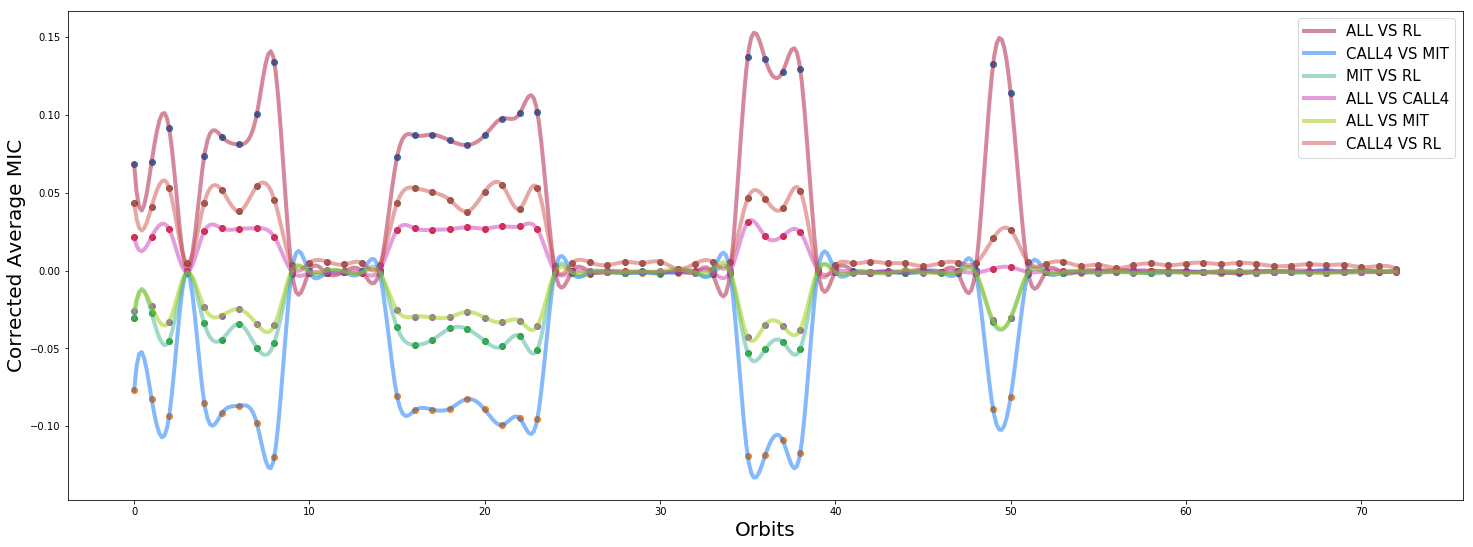
\includegraphics[width=\textwidth]{figures/orbits_correlations_all.png}
    \caption{
        \textbf{Pair-wise average orbit correlations:}
        In figure \ref{fig:orbits_correlations_all}, each point
        in the graph is the result of averaging pair-wise
        orbit correlations over all contact maps
        ($\frac{1}{276}\sum_{i=0}^{23}\sum_{j=i}^{23}{
        m^{\scriptscriptstyle \scriptscriptstyle A,B}_{i,j, o}} \quad 
        \forall o \in \{0, 1, ..., 72\}$:
        average along the red \textit{horizontal} arrows in figure 
        \ref{graphlet_correlation_schema}).
        Counts for certain orbits are always zero in inter-chromosomal
        maps, leading to average value close to zero in 
        Figure \ref{fig:orbits_correlations_all}.
        In this figure, cancer cells data points are depicted
        in warm colors while normal cells are depicted in
        cold colors in increased contrast. As can be seen
        orbit distributions are more similar to each other
        for cancer cells.
    }
    \label{fig:orbits_correlations_all}
\end{figure*}


\subsection{Statistical Analysis}
In order to qauntify our results, we have conducted one-sided
t-test in order to test whether the average pair-wise
MIC values across orbits are significantly different from 
each other and also from 1. 
however, pairwise correlation of cancer cells for
orbits in $\mathbb{Q}$ were significantly higher than
correlation between cancer cells and normal cells.
The results
for this test showed that all values are significantly less than 1;
A summary of can be found in
table \ref{tab:t-test}.
We have also conducted t-tests for 
pair-wise orbit signature vector distances across contact maps.
Please refer to supplementary material for result of the 
full list of t-test results.
\begin{table}[H]
    \resizebox{.5\textwidth}{!}{
\begin{tabular}{c|ccccccc}
    & $MIC_{\scriptscriptstyle MIT-CALL4}$ & $MIC_{\scriptscriptstyle MIT-RL}$ & $MIC_{\scriptscriptstyle MIT-ALL}$ & $MIC_{\scriptscriptstyle ALL-CALL4}$ & $MIC_{\scriptscriptstyle CAll4-RL}$ & $MIC_{\scriptscriptstyle ALL-RL}$ & 1   \\
              \rule{0pt}{1pt} \\ \hline \rule{0pt}{15pt}
              $MIC_{\scriptscriptstyle MIT-CALL4}$ & -         & $\mathbf{<}$    & $\mathbf{<}$     & $\mathbf{<}$       & $\mathbf{<}$      & $\mathbf{<}$    & $\mathbf{<}$ \\
              \rule{0pt}{20pt}
              $MIC_{\scriptscriptstyle MIT-RL}$    & $\mathbf{>}$       &   -    & $\mathbf{<}$     & $\mathbf{<}$       & $\mathbf{<}$      & $\mathbf{<}$    & $\mathbf{<}$ \\
              \rule{0pt}{20pt}
              $MIC_{\scriptscriptstyle MIT-ALL}$   & $\mathbf{>}$       & $\mathbf{>}$    &    -    & $\mathbf{<}$       & $\mathbf{<}$      & $\mathbf{<}$    & $\mathbf{<}$ \\
              \rule{0pt}{20pt}
              $MIC_{\scriptscriptstyle ALL-CALL4}$ & $\mathbf{>}$       & $\mathbf{>}$    & $\mathbf{>}$     &       -   & $\mathbf{<}$      & $\mathbf{<}$    & $\mathbf{<}$ \\
              \rule{0pt}{20pt}
              $MIC_{\scriptscriptstyle CAll4-RL}$  & $\mathbf{>}$       & $\mathbf{>}$    & $\mathbf{>}$     & $\mathbf{>}$       &    -     & $\mathbf{<}$    & $\mathbf{<}$ \\
              \rule{0pt}{20pt}
              $MIC_{\scriptscriptstyle ALL-RL}$    & $\mathbf{>}$       & $\mathbf{>}$    & $\mathbf{>}$     & $\mathbf{>}$       & $\mathbf{>}$      &   -    & $\mathbf{<}$ \\
              \rule{0pt}{20pt}
              1         & $\mathbf{>}$       & $\mathbf{>}$    & $\mathbf{>}$     & $\mathbf{>}$       & $\mathbf{>}$      & $\mathbf{>}$    &    -
\end{tabular}}
    \caption{
        Result of one-sided t-test 
        comparison of MIC results 
        with significance $\alpha = 0.01$
        for orbits of $\mathbb{Q}$.
        A $<$ sign means that the value in the corresponding
        row is significantly smaller that the value in 
        corresponding column; and a $>$ sign means the opposite.
        An $=$ sign would have meant the values are not 
        statistically different.
        As can be seen, all MIC values are significantly smaller that 1,
        meaning non on them are exactly the same; 
        however, all Cancer vs Cancer MIC values are statistically
        larger than Cancer vs Normal, implying that 
        spatial positioning of loci are more similar between cancer cells.
    }
    \label{tab:t-test}

\end{table}

\section{Resources}
\textbf{Hi-C Datasets:}
\begin{enumerate}
    \item \href{https://github.com/rasoolianbehnam/watson}{Code base for this article}
    \item \href{http://sysbio.rnet.missouri.edu/T0510/tmp_download/link_to_download_genome_data/}
        {Datasets including cancerous cells}
    \item \href{https://bcm.app.box.com/v/aidenlab/folder/11234760671}{Original Datasets}
\end{enumerate}

\bibliography{lit}
\bibliographystyle{unsrt}
\end{document}
